\documentclass[a4paper, 10pt, spanish]{article}

\usepackage[paper=a4paper, left=1.5cm, right=1.5cm, bottom=1.5cm, top=3.5cm]{geometry}
\usepackage[spanish, es-noshorthands]{babel}
\usepackage[utf8x]{inputenc}
\usepackage[none]{hyphenat}
\usepackage[colorlinks,citecolor=black,filecolor=black,linkcolor=black,    urlcolor=black]{hyperref}

% Simbolos matemáticos
\usepackage{amsthm}
\usepackage{amsmath}
\usepackage{amsfonts}
\usepackage{amssymb}
\usepackage{algorithm}
\usepackage[noend]{algpseudocode}
\usepackage{algorithmicx}
\usepackage{listings}
\usepackage{enumerate}

% Descoración y gráficos
\usepackage{caratulaV}
\usepackage{graphicx} 
\usepackage{fancyhdr}
\usepackage{lastpage}
\usepackage{caption}
\usepackage{subcaption}
\usepackage{multirow}
\usepackage{alltt}
\usepackage{tikz}
\usepackage{varwidth,xcolor}
\usepackage{color}
\usepackage{gnuplottex}
\usepackage{verbatim}
\usepackage{framed}


% Del enunciado
\usepackage{a4wide}
\usepackage{amsmath}
\usepackage{amsfonts}
%\usepackage[ruled,vlined]{algorithm2e}

\newcommand{\kknn}{k}
\newcommand{\kpca}{\alpha}
\newcommand{\kkfold}{K}

% Acomodo fancyhdr.
\pagestyle{fancy}
\thispagestyle{fancy}
\addtolength{\headheight}{1pt}
\lhead{Sistemas operativos}
\rhead{$2^{\mathrm{do}}$ cuatrimestre de 2015}
\cfoot{\thepage /\pageref*{LastPage}}
\renewcommand{\footrulewidth}{0.4pt}

\floatname{algorithm}{Pseudocodigo}
\algrenewcommand\algorithmicfunction{\textbf{Funcion}}
\algrenewcommand\algorithmicwhile{\textbf{mientras}}
\algrenewcommand\algorithmicfor{\textbf{para}}
\algrenewcommand\algorithmicforall{\textbf{para cada}}
\algrenewcommand\algorithmicdo{\textbf{hacer:}}
\algrenewcommand\algorithmicif{\textbf{si}}
\algrenewcommand\algorithmicthen{\textbf{entonces:}}
\algrenewcommand\algorithmicelse{\textbf{si no:}}
\algrenewcommand\algorithmicend{\textbf{fin}}
\algrenewcommand\algorithmicreturn{\textbf{devolver}}



\sloppy

\parskip=5pt % 10pt es el tama de fuente

% Pongo en 0 la distancia extra entre itemes.
\let\olditemize\itemize
\def\itemize{\olditemize\itemsep=0pt}



\usepackage{tikz}
%\usepackage{tikz-qtree}


\usetikzlibrary{arrows,backgrounds,calc}

\pgfdeclarelayer{background}
\pgfsetlayers{background,main}

\newcommand{\real}{\mathbb{R}}
\newcommand{\nat}{\mathbb{N}}

\newcommand{\revJ}[1]{{\color{red} #1}}

\newcommand{\convexpath}[2]{
[ 
    create hullnodes/.code={
        \global\edef\namelist{#1}
        \foreach [count=\counter] \nodename in \namelist {
            \global\edef\numberofnodes{\counter}
            \node at (\nodename) [draw=none,name=hullnode\counter] {};
        }
        \node at (hullnode\numberofnodes) [name=hullnode0,draw=none] {};
        \pgfmathtruncatemacro\lastnumber{\numberofnodes+1}
        \node at (hullnode1) [name=hullnode\lastnumber,draw=none] {};
    },
    create hullnodes
]
($(hullnode1)!#2!-90:(hullnode0)$)
\foreach [
    evaluate=\currentnode as \previousnode using \currentnode-1,
    evaluate=\currentnode as \nextnode using \currentnode+1
    ] \currentnode in {1,...,\numberofnodes} {
-- ($(hullnode\currentnode)!#2!-90:(hullnode\previousnode)$)
  let \p1 = ($(hullnode\currentnode)!#2!-90:(hullnode\previousnode) - (hullnode\currentnode)$),
    \n1 = {atan2(\x1,\y1)},
    \p2 = ($(hullnode\currentnode)!#2!90:(hullnode\nextnode) - (hullnode\currentnode)$),
    \n2 = {atan2(\x2,\y2)},
    \n{delta} = {-Mod(\n1-\n2,360)}
  in 
    {arc [start angle=\n1, delta angle=\n{delta}, radius=#2]}
}
-- cycle
}

\newcommand{\todo}[1]{
\textbf{\color{red}{\underline{Nota:} #1}}
}

\newcommand\param[3]{\ensuremath{\mathbf{\textbf{#1}}\,#2\!:} \texttt{#3}}

\let\state\State
\let\while\While
\let\endwhile\EndWhile
\let\endif\EndIf
\let\elseif\ElsIf
\let\for\For
\let\endfor\EndFor
\let\function\Function
\let\endfunction\EndFunction


\newcommand{\degree}{\ensuremath{^\circ}}

\begin{document}
%\setcounter{tocdepth}{2}
\renewcommand{\tablename}{Tabla} 


\thispagestyle{empty}
\materia{Sistemas operativos}
\submateria{Segundo Cuatrimestre de 2015}
\titulo{Trabajo Práctico I}

\integrante{Federico De Rocco }{403/13}{fede.183@hotmail.com}
\integrante{Fernando Otero}{424/11}{fergabot@gmail.com}
\integrante{Carmen Premuzic}{408/98}{asdlkj.1209@gmail.com}

\maketitle
\newpage
%\begin{titlepage}

%\maketitle

%\end{titlepage}
\setcounter{page}{1}

\newpage
\tableofcontents

\newpage
%\input{desarrollo}

\newpage


\section{Ejercicio 1}


\subsection{Desarrollo}
Sabiendo que la tarea solamente se dedica a bloquearse una cantidad n de veces y con una duración al azar entre bmin y bmax, lo que hacemos para resolver este ejercicio es 
simplemente conseguirnos un número aleatorio n veces. Para esto usamos la función de c++ rand(), aclarando que queremos que los valores se encuentren entre los pedidos.

\subsection{Experimentación}
Para cumplir con lo pedido en el ejercicio utilizaremos el lote de tareas loteEj1.tsk, la representación del mismo usando la política FCFS es la siguiente:


\begin{figure}[H]
  \centering
    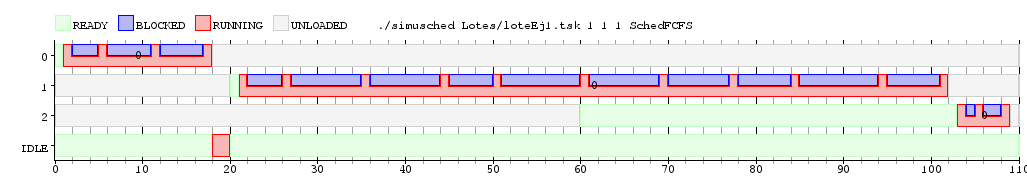
\includegraphics[width=1.1\textwidth]{imagenes/Ex1Ej1.png}
  \caption{loteEj1.tsk con FCFS}
\end{figure}

Con este gráfico podemos ver como, para cada una de las tres tareas, van apareciendo varias llamadas bloqueantes de una duración diferente las unas de las otras. Considerando 
que la cantidad para cada una (especificada por el primer parámetro, n) es correcta y que el tiempo de las llamadas está entre los elegidos, podemos decir que el algoritmo es correcto.

\begin{figure}[H]
  \centering
    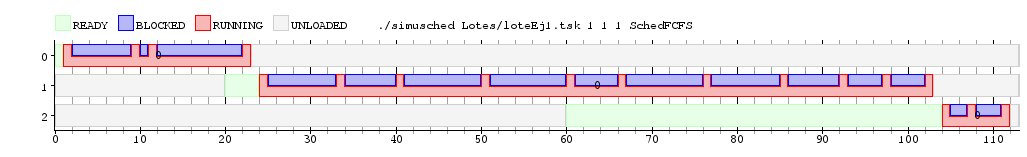
\includegraphics[width=1.1\textwidth]{imagenes/Ex2Ej1.png}
  \caption{loteEj1.tsk con FCFS}
\end{figure}

Ejecutamos, por segunda vez, en las mismas condiciones para mostrar como varían los tiempos de los bloqueos.

\section{Ejercicio 2}


\subsection{Experimentación}
El loteEj2.tsk contiene lo pedido por enunciado.

TaskCPU 100  

TaskConsola 20 2 4

TaskConsola 25 2 4

Veamos que tiene un uso de 100 de cpu que es del algoritmo complejo, un TaskConsola que es para la canción que realiza 20 llamadas bloqueantes y el otro de 25 para navegar por
internet. Las llamadas bloqueantes son entre 2 y 4.

\begin{figure}[H]
  \centering
    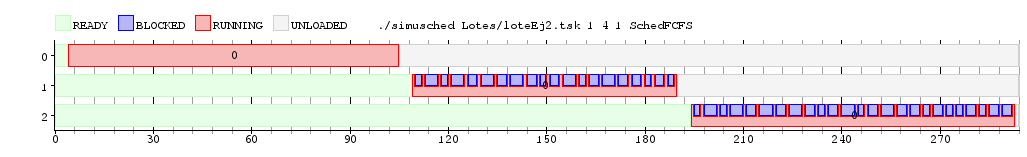
\includegraphics[width=1.1\textwidth]{imagenes/Ej2Experimento1core.png}
  \caption{loteEj2.tsk con FCFS y coste cambio de contexto de 4 ciclos con 1 núcleo}
\end{figure}

\begin{tabular}{l | r }
  Proceso & Latencia\\
  \hline
  CPU & 4\\
  Canción favorita & 108\\
  Navegar por Internet & 194\\
\end{tabular}

\begin{figure}[H]
  \centering
    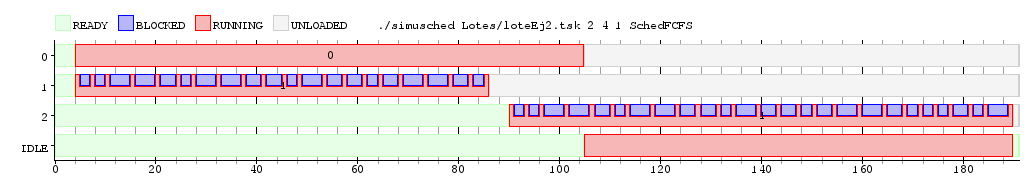
\includegraphics[width=1.1\textwidth]{imagenes/Ej2Experimento2core.png}
  \caption{loteEj2.tsk con FCFS y coste cambio de contexto de 4 ciclos con 2 núcleo}
\end{figure}

\begin{tabular}{l | r }
  Proceso & Latencia\\
  \hline
  CPU & 4\\
  Canción favorita & 4\\
  Navegar por Internet & 91\\
\end{tabular}

Hay que aclarar que las latencias podrían variar ya que TaskConsola genera las llamadas bloqueantes con un tamaño aleatorio entre 2 y 4. Podemos ver que en el primer caso se
debe esperar hasta que el algoritmo complejo termine para poder escuchar musica y , a su vez, que esto termine para poder navegar por internet. En el segundo caso, vemos que 
se puede ejecutar el algoritmo complejo y escuchar la canción al mismo tiempo, pero se debe terminar la canción para poder navegar por internet. Este último es mejor porque
la canción y navegar por internet tienen latencias menores. 

Rolando va a tener muchos problemas para ejecutar esto con un solo núcleo ya que mientras se este ejecutando el cpu no se podrá hacer ninguna de las otras cosas, que es lo que él
pretende. Una buena solución sería tener 3 núcleos para que las tres cosas se puedan hacer al mismo tiempo. Otra sería usar Round-Robin para poder ir alternando los procesos y 
que no tenga que esperar que uno termine para poder ir ejecutando los otros.

\section{Ejercicio 3}

\subsection{Desarrollo}
Para poder resolver el problema de TaskBatch lo que hacemos es generar cant$\_$bloqueos valores aleatorios no repetidos que no estén ubicados fuera de total$\_$cpu. 
Lo generado por esto podría no estar ordenado, así que le hacemos un sort al resultado. Por último ciclaremos total$\_$cpu veces y en las posiciones donde se tendría que 
bloquear hacemos la llamada usa$\_$IO con duración de 1.

\subsection{Experimentación}
Siguiendo lo pedido por enunciado, realizaremos el gráfico del loteEj3.tsk usando el FCFS y nos queda lo siguiente:

\begin{figure}[H]
  \centering
    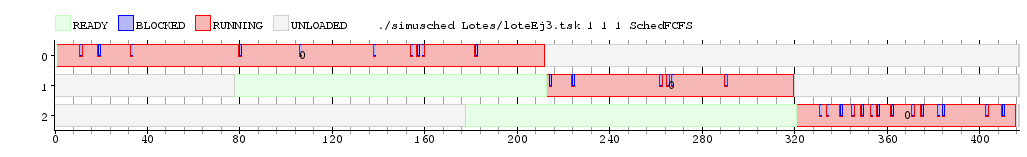
\includegraphics[width=1.1\textwidth]{imagenes/BatchExperimento.png}
  \caption{loteEj3.tsk con FCFS}
\end{figure}
\section{Ejercicio 4}

\subsection{Desarrollo}
El ejercicio consiste en programar un scheduler de Round-Robin, para esto utilizaremos las siguientes estructuras: vector de enteros pid$\_$cores, vector de booleanos cores$\_$bloqueados, vector de enteros quantum$\_$restantes, entero cant$\_$cores, entero cpu$\_$quantum, Una cola de enteros enEspera.

Cuando creamos el scheduler se nos dan la cantidad de cores(que será cant$\_$cores) y el quantum de los cpus(cpu$\_$quantum). Segun el enunciado los procesos están agrupados en una única cola, de ahí viene enEspera. Como conocemos la cantidad de cores usamos tres estructuras de vectores para, solo teniendo el numero del cpu, poder acceder a la información de las mismas. cores$\_$bloqueados nos indica si el proceso del núcleo en cuestión está o no bloqueado, pid$\_$cores nos da el pid del proceso que esta corriendo en el cpu y quantum$\_$restantes nos dice cuanto tiempo le queda por ejecutar hasta terminar.
En el programa load en el cual tenemos que poner un proceso en el scheduler lo que haremos será buscar si hay algún core en pid$\_$cores que tenga cargada la tarea IDLE.
 
Si lo encontramos, cargamos el proceso en ese core poniéndolo en pid$\_$cores y dándole al quantum$\_$restantes de ese proceso el valor de cpu$\_$quantum ya que es una tarea que está por comenzar a ejecutar. Caso contrario, simplemente lo encolamos en enEspera para ser ejecutada cuando sea su turno.
En el caso de unblock lo que hacemos es buscar entre los cores cual es el que tiene cargado el proceso que se desea bloquear(en pid$\_$cores), una vez encontrado acceder a su posición en cores$\_$bloqueados y asignarle true.
Por último tenemos el programa tick que se encarga de realizar los procedimientos pertinentes en cada tick de reloj. Tenemos tres casos de motivos:
 
TICK: en el mismo sabemos que ha pasado un tick de reloj y debemos disminuir los cuantos que le quedan al procedimiento del cpu. En el caso de que estos terminen en 0 debemos plantearnos si debemos desalojar la tarea para poner otra. Si se da el caso de que el proceso está bloqueado entonces no realizamos ninguno de estos procesos ni disminuimos el quantum.

BLOCK: Disminuimos el quantum restante y bloqueamos el core(poniendo true en cores$\_$bloqueados).

EXIT: Colocamos en el core la tarea IDLE y si la cola no está vacía, le asignamos la tarea que se encuentre próxima en ella. Después reseteamos los quantum del proceso. 


\subsection{Experimentación}
Para poder probar el correcto funcionamiento de la estructura se realizo una serie de experimentos, los mismos consisten en ejecutar el schedule con distintos lotes de tareas que poseemos, también variamos la cantidad de cores. 

\section{Ejercicio 5}


\subsection{Desarrollo}
En el ejercicio se pide diseñar un lote con tres tareas de 50 ciclos y dos de 5 llamadas bloqueantes de 3 ciclos de duración. El lote que representamos inicia todas las tareas a la vez
\begin{verbatim}
TaskCPU 50
TaskCPU 50
TaskCPU 50
TaskConsola 5 3 3
TaskConsola 5 3 3
\end{verbatim}
Se pide calcular latencia, waiting time y tiempo total de ejecución 
\subsection{Experimentación}
\begin{figure}[H]
  \centering
    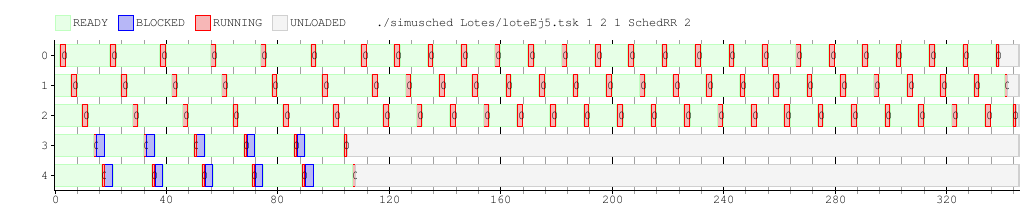
\includegraphics[width=1.1\textwidth]{imagenes/Ej5_q2.png}
  \caption{loteEj5.tsk con RR y quantum 2}
\end{figure}
\begin{figure}[H]
  \centering
    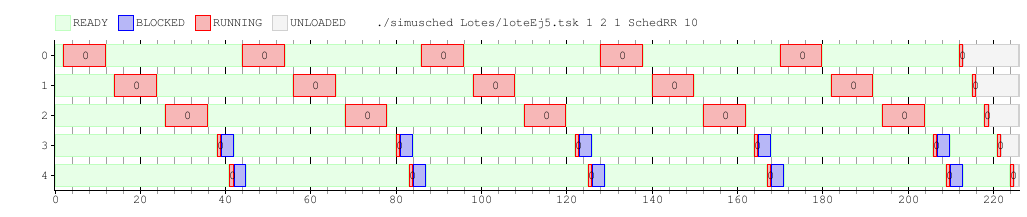
\includegraphics[width=1.1\textwidth]{imagenes/Ej5_q10.png}
  \caption{loteEj5.tsk con RR y quantum 10}
\end{figure}
\begin{figure}[H]
  \centering
    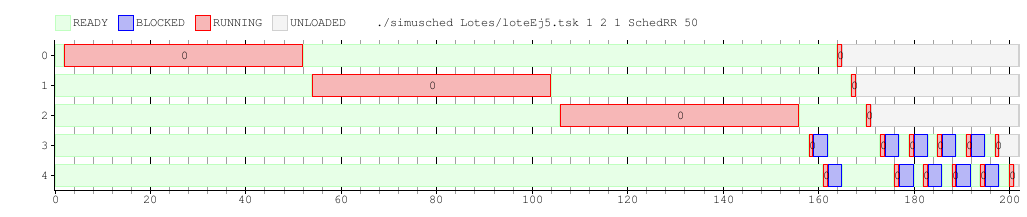
\includegraphics[width=1.1\textwidth]{imagenes/Ej5_q50.png}
  \caption{loteEj5.tsk con RR y quantum 50}
\end{figure}
\paragraph{quantum: 2}\par
\begin{tabular}{ l | c | c | c | c | c | c | }
  \hline			
  pid & ciclos & inicio & fin & latencia & waiting time & tiempo total  \\
  \hline
 0 & 51 & 0 & 339 & 2 & 288 & 339\\
1 & 51 & 0 & 342 & 6 & 291 & 342\\
2 & 51 & 0 & 345 & 10 & 294 & 345\\
3 & 21 & 0 & 105 & 14 & 84 & 105\\
4 & 21 & 0 & 108 & 17 & 87 & 108\\
  \hline
\end{tabular}
\paragraph{quantum: 10}\par
\begin{tabular}{ l | c | c | c | c | c | c | }
  \hline			
  pid & ciclos & inicio & fin & latencia & waiting time & tiempo total  \\
  \hline
0 & 51 & 0 & 213 & 2 & 162 & 213\\
1 & 51 & 0 & 216 & 14 & 165 & 216\\
2 & 51 & 0 & 219 & 26 & 168 & 219\\
3 & 21 & 0 & 222 & 38 & 201 & 222\\
4 & 21 & 0 & 225 & 41 & 204 & 225\\
\hline
\end{tabular}
\paragraph{quantum: 50}
\begin{tabular}{ l | c | c | c | c | c | c | }
  \hline			
  pid & ciclos & inicio & fin & latencia & waiting time & tiempo total  \\
  \hline
0 & 51 & 0 & 165 & 2 & 114 & 165\\
1 & 51 & 0 & 168 & 54 & 117 & 168\\
2 & 51 & 0 & 171 & 106 & 120 & 171\\
3 & 21 & 0 & 198 & 158 & 177 & 198\\
4 & 21 & 0 & 201 & 161 & 180 & 201\\
  \hline
\end{tabular}

\section{Ejercicio 6}


\subsection{Desarrollo}



\subsection{Experimentación}

\section{Ejercicio 7}


\subsection{Desarrollo}



\subsection{Experimentación}

\section{Ejercicio 8}


\subsection{Desarrollo}
Similar  a lo visto en el ejercicio 4, tendremos que programar la estructura de un scheduler de Round-Robin. La diferencia es que en este caso en vez de tener una cola única 
que vaya guardando todos los procesos, cada core tendrá su propia cola de procesos. Para resolver esto utilizaremos una estructura para representar el core que nos dará la 
siguiente información: un entero pidActual, un entero cpu$\_$quantum, un entero quantum$\_$restantes, su cola de pids enEspera, un vector pid$\_$bloqueados que indica cuales están en ese estado.

Después tenemos la cantidad de cores y el quantum de los mismos. Por último necesitamos agrupar las estructuras core que tenemos. Para esto usamos simplemente un vector 
(nucleos).

La función load lo que hace es buscar cual de los cores tiene menor cantidad de procesos(suma los bloqueados, los de enEspera y el de pidActual, si no es IDLE). Una vez 
encontrado, lo encola en el enEspera del core.

unblock lo que hace es buscar cual es el core donde se encuentra el pid que se desea bloquear, una vez encontrado lo quita de pid$\_$bloqueados y lo pone en enEspera.

Por último tenemos la función tick. El código es equivalente al del ejercicio 4.


\subsection{Experimentación}
Según lo pedido debemos mencionar un caso donde la migración de núcleos sea beneficiosa y otro donde no. Para lo primero, usaremos dos core y cuatro tareas que irán apareciendo
en este orden: la más costosa,  la menos costosa, la segunda más costosa y la segunda menos costosa. Usaremos, en los dos cores, un quantum de 5(para todos) y nos queda lo siguiente:

TaskCPU 100   	//Costosa

@1:

TaskCPU 10 	//Poco Costosa

@2:

TaskCPU 80 	//Costosa

@3:

TaskCPU 20 	//Poco Costosa

\begin{figure}[H]
  \centering
    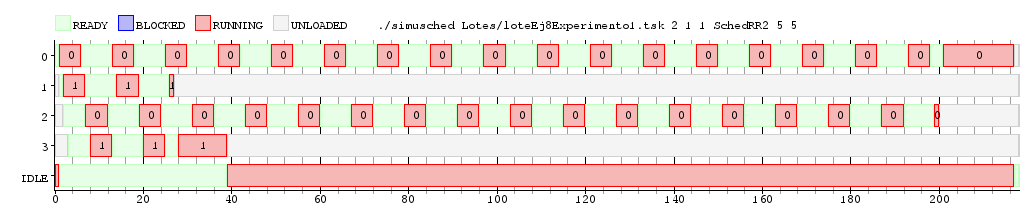
\includegraphics[width=1.1\textwidth]{imagenes/Ej8Experimento1.png}
  \caption{loteEj8Experimento1.tsk con RR}
\end{figure}

\begin{tabular}{l | r | r | r }
  Proceso & Latencia & Waiting time & Tiempo total\\
  \hline
  Tarea 0 & 1 & 30 & 131 \\
  Tarea 1 & 1 & 15 & 26 \\
  Tarea 2 & 5 & 28 &  109\\
  Tarea 3 & 5 & 30 & 51\\
  Promedio & 3 & 25.75 & 79.25\\
\end{tabular}

\begin{figure}[H]
  \centering
    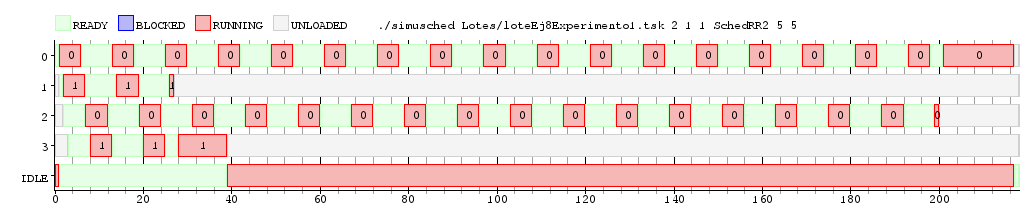
\includegraphics[width=1.1\textwidth]{imagenes/Ej8Experimento2.png}
  \caption{loteEj8Experimento1.tsk con RR2}
\end{figure}

\begin{tabular}{l | r | r | r }
  Proceso & Latencia & Waiting time & Tiempo total\\
  \hline
  Tarea 0 & 1 & 116 &  216\\
  Tarea 1 & 1 & 15 &  22\\
  Tarea 2 & 5 & 117 & 198 \\
  Tarea 3 & 5 & 15 & 36\\
  Promedio & 3 & 65.75 & 118 \\
\end{tabular}

Podemos ver que la corrida con el RR2 tarda más en terminar las tareas más costosa respecto a lo que tarda RR(todas excepto la Tarea 1). Esto se debe a que solo son atendidas 
por un cpu mientras el otro ejecuta tareas de bajo costo y, por lo tanto, termina antes y se queda inactivo mientras el otro sigue trabajando. Mientras tanto el que posee 
migración de núcleos. 
Las más costosas tienen un peor waiting time. También se ve que tiempo final promedio y el waiting time promedio es mayor en la que no tiene migración de núcleos. Por
lo tanto para este lote es mejor el scheduler con migración de núcleos. 

Para el caso donde es peor utilizaremos el siguiente lote de tareas:

TaskCPU 100

@6:

TaskCPU 30

@12:

TaskCPU 30

El cambio es que las ejecuciones tendrán un costo de migración de núcleos de 10(en los anteriores experimentos era de 1).

\begin{figure}[H]
  \centering
    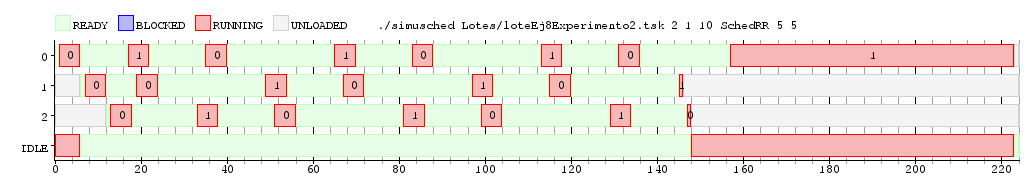
\includegraphics[width=1.1\textwidth]{imagenes/Ej8Experimento3.png}
  \caption{loteEj8Experimento2.tsk con RR}
\end{figure}

\begin{tabular}{l | r | r | r }
  Proceso & Latencia & Waiting time & Tiempo total\\
  \hline
  Tarea 0 & 1 & 122 &  223\\
  Tarea 1 & 1 & 109 &  140\\
  Tarea 2 & 5 & 105 & 132 \\
  Promedio & 2.33 & 112 & 165 \\
\end{tabular}

\begin{figure}[H]
  \centering
    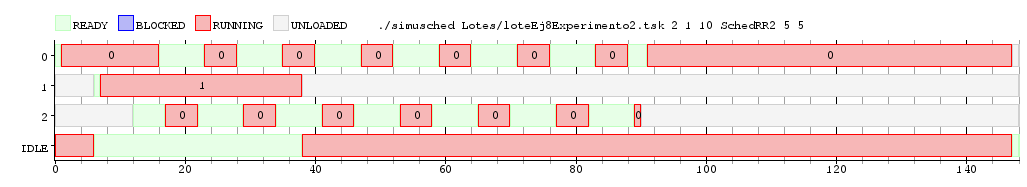
\includegraphics[width=1.1\textwidth]{imagenes/Ej8Experimento4.png}
  \caption{loteEj8Experimento2.tsk con RR2}
\end{figure}

\begin{tabular}{l | r | r | r }
  Proceso & Latencia & Waiting time & Tiempo total\\
  \hline
  Tarea 0 & 1 & 46 &  147\\
  Tarea 1 & 1 & 1 &  32\\
  Tarea 2 & 5 & 47 & 78 \\
  Promedio & 2.33 & 31.33 & 85.66 \\
\end{tabular}

Podemos ver que, en este caso, el waiting time promedio y el tiempo total promedio son mejores en el que no tiene migración de núcleos. Esto es debido a que el scheduler RR2
no paga el costo de migración porque cada tarea se ejecuta siempre en el mismo núcleo, mientras que RR cada vez que desaloja una tarea tarda más tiempo si la próxima no se estuvo
ejecutando en el mismo core. El lote esta pensado para que esto suceda.



\newpage

\ref{LastPage}

\end{document}
